\documentclass{beamer}
%\usetheme{Ilmenau}
%\usecolortheme{beaver}

\usepackage[slovak,american]{babel}
\usepackage[utf8]{inputenc}
\usepackage{graphicx}
\usepackage{adjustbox}
 \usepackage{xcolor}
 
 \newsavebox\MBox
\newcommand\Cline[2][red]{{\sbox\MBox{$#2$}%
  \rlap{\usebox\MBox}\color{#1}\rule[-2.2\dp\MBox]{\wd\MBox}{1pt}}}

%\usefonttheme{serif}

\definecolor{UKOrange}{HTML}{ef9424} %
\definecolor{UKBrown}{HTML}{a96d5e} %
\definecolor{UKLight}{HTML}{d8b6ab} %
\definecolor{UKDark}{HTML}{7a4f44}
\definecolor{UKDarker}{HTML}{4d312b} 
\definecolor{UKDarkest}{HTML}{2e1e1a}
\definecolor{UKRed}{HTML}{bf1f1c}

\setbeamertemplate{footline}[frame number]{}
\setbeamertemplate{navigation symbols}{}

%\usecolortheme{beaver}
\setbeamertemplate{itemize item}[square]
\setbeamercolor{itemize item}{fg = UKBrown}
\setbeamercolor{itemize subitem}{fg = UKLight}
\setbeamercolor{enumerate item}{fg = UKDark}

\setbeamercolor{footnote}{fg=UKLight}
\setbeamercolor{footnote mark}{fg=UKLight}
\setbeamerfont{footnote}{size=\tiny}
\renewcommand\footnoterule{}

\usetheme{default}
\beamertemplatenavigationsymbolsempty
\setbeamercolor{title}{fg=white, bg=UKBrown}
\setbeamercolor{frametitle}{fg=white, bg=UKBrown}
\setbeamercolor{block title}{bg=UKBrown, fg= white}
\setbeamercolor{block body}{bg =UKLight, fg = UKDarkest}

\useoutertheme[subsection=false]{miniframes}
\AtBeginSection[]{\subsection{}}

\setbeamercolor{below lower separation line head}{bg=UKDark}
\addtobeamertemplate{headline}{}{%
  \begin{beamercolorbox}[colsep=0.5pt]{below lower separation line head}
  \end{beamercolorbox}
}
%\setbeamercolor*{mini frame}{fg=white,bg=UKRosy}
\setbeamercolor{section in head/foot}{fg=UKLight, bg=UKDark}

%\setbeamertemplate{itemize/enumerate body begin}{\normalsize}
%\setbeamertemplate{itemize/enumerate subbody begin}{\normalsize}




%\newcommand{\codeblock}[2]{ \begin{block}{#1} \begin{verbatim}#2\end{verbatim}\end{block}}

%\defbeamertemplate*{title page}{customized}[1][]
%{
%  \begin{centering}
%    \begin{beamercolorbox}[sep=8pt,center]{title}
%      \usebeamerfont{title}\inserttitle
%    \end{beamercolorbox}
%  \end{centering}
%  \bigskip
%
%\begin{columns}[onlytextwidth,T]
%
%
%  \column{27mm}
%  \includegraphics[width=27mm]{images/logoFMFI.png}
%  
%  \column{\dimexpr\linewidth-54mm-6mm}
%  \centering
%  \vspace{5mm}  
%  \usebeamerfont{author}\insertauthor\par
%  \vspace{5mm}
%  \usebeamerfont{institute}\insertinstitute\par
%
%  \column{27mm}
%  \includegraphics[width=27mm]{images/logoUK.png}  
%\end{columns}
%\centering
%\vspace{7mm}
%  \usebeamerfont{date}\insertdate\par
%}


\title[PCA a LDA]{Rozpoznávanie obrazcov - 4. cvičenie \\ Redukcia dimenzionality}
\author[Viktor Kocur]{Viktor Kocur \\{\small viktor.kocur@fmph.uniba.sk}}
\institute{DAI FMFI UK}
\date{19.3.2019}
%\titlegraphic{\includegraphics[width=2.7cm]{images/logoFMFI.png}\hspace*{1cm}~%
%   \includegraphics[width=2.7cm]{images/logoUK.png}
%}


\begin{document}
\selectlanguage{slovak}

\begin{frame}[plain]
  \titlepage  
\end{frame}

\section{PCA}

\begin{frame}
\frametitle{PCA princíp}
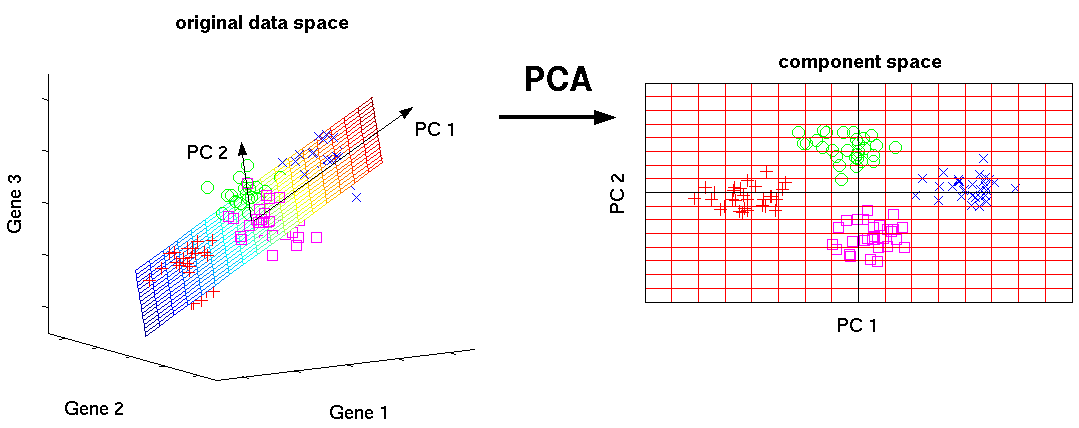
\includegraphics[width=\textwidth]{PCA.png}
\end{frame}


\begin{frame}
\frametitle{PCA motivácia}
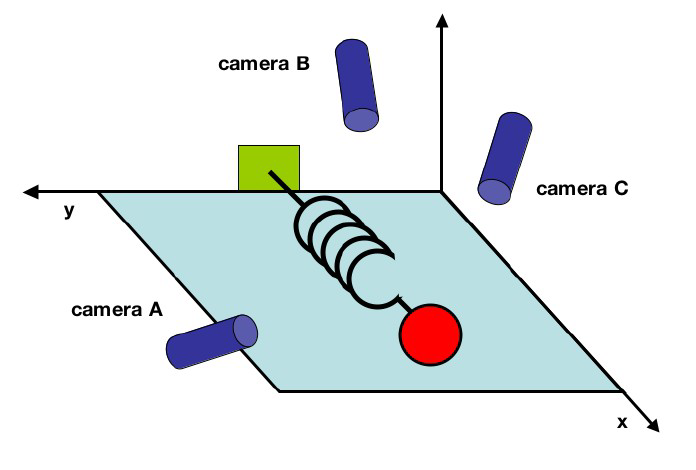
\includegraphics[width=\textwidth]{PCAcameras.png}
\end{frame}


\begin{frame}
\frametitle{PCA matematika}

\begin{block}{Eigenvectors and eigenvalues}
Let $\mathbb{A}$ be a matrix $n \times n$, then a nonzero vector $\vec{v} \in \mathbb{R}^n$ is an eigenvector of $\mathbb{A}$ with eigenvalue $\lambda \in \mathbb{C}$ if: $\mathbb{A}\vec{v} = \lambda \vec{v}$. 
\end{block}

\begin{block}{Hermitian Matrix}
Hermitian matrices have only real eigenvalues. It is also possible to find an eigenvector for each eigenvalue.
\end{block}
\end{frame}


\begin{frame}
\frametitle{PCA theory}

\begin{block}{Covariance}
$cov (X, Y) = \frac{\sum_{i=1}^n (X_i - \overline{X})(Y_i - \overline{Y})}{n}$
\end{block}

\begin{block}{Covariance matrix}
$COV(X)_{i,j} = cov(X_i, X_j)$
\end{block}

\begin{block}{Covariance matrix}
Covariance matrix is Hermitian and positively semi-definite.
\end{block}
\end{frame}



\begin{frame}
\frametitle{PCA theory}

\begin{block}{Matrix of eigenvectors}
Z normalizovaných vlastných čísel $v_1 ... v_n$ zostavíme maticu $(v_1, v_2, ... , v_n)$. Značíme $\mathbb{W}$.
\end{block}

\begin{block}{PCA}
PCA is based on the fact that eigenvectors of covariance matrix represent an orthogonal base in which the covariance matrix is diagonal.
\end{block}

\begin{block}{PCA process}
We start by centering our data as $\vec{x}' = \vec{x} - \overline{x}$. Then we compute $\mathbb{W}$. The new data are obtained by matrix multiplication $ y = \vec{x}' \mathbb{W}^T$, if $\vec{x}$ is a row vector. Eigenvalues correspond to the portion of the variance explained by given direction.
\end{block}
\end{frame}



\begin{frame}
\frametitle{Matlab}

\begin{block}{Loading data}
load data.mat
\end{block}

\begin{block}{Exercise}
Display 2D data in a plot.
\end{block}

\end{frame}


\begin{frame}
\frametitle{Matlab functions}

\begin{block}{cov}
cov(A) - returns covariance matrix of A
\end{block}

\begin{block}{eig}
[W, vals] = eig(A) - return matrix W with eigenvectors W and eigenvalues on the diagonals of matrix vals for matrix A.
\end{block}

\begin{block}{Exercise}
Apply PCA on the data and plot the transformed data. Show how much variance is explained by each direction.
\end{block}
\end{frame}

\begin{frame}[fragile]
\frametitle{Solution}
\begin{verbatim}
load data.mat
plot(data(:,1), data(:,2), 'r*');
centered = data - mean(data);
[W, eigenvals] = eig(cov(centered))
newdata = centered * W'
plot(newdata(:,1), newdata(:,2), 'r*');
ylim([-2 2]);
xlim([-2 2]);
disp(diag(eigenvals)/sum(diag(eigenvals)))
\end{verbatim}
\end{frame}

\begin{frame}
\frametitle{Matlab - PCA function}

\begin{block}{cov}
[coeff,score,~,~,explained,mu] = pca(X) - returns transformation matrix coeff (we denote as $\mathbb{W}^T$), transformed data in score, percentages of variance explained by different directions and mean values of X.

\end{block}

\begin{block}{Transformation}
score == (X - mu) * coeff
\end{block}

\begin{block}{Inverse transformation}
X == score * coeff' + mu
\end{block}

\begin{block}{Exercise}
Test this function on data.mat.
\end{block}

\end{frame}

\begin{frame}
\frametitle{Matlab - PCA}

\begin{block}{Data}
load ovariancancer
\end{block}

\begin{block}{gscatter}
gscatter(obs(:,1), obs(:,2), grp) - displays points from the first two columns of the dataset and shows the color based on grp class.
\end{block}

\begin{block}{Exercise}
Determine how many features (dimensions after transformation) do you need to keep at least 95 percent of variance of the dataset. What does it mean if some eigenvalues are zeros?
\end{block}

\begin{block}{Exercise}
Show the plot for 2 most significant dimensions of the data after PCA using gscatter.
\end{block}
\end{frame}


\begin{frame}
\frametitle{PCA - exercises}

\begin{block}{Exercise}
For data from data.mat show the directions to which we project the data in the original coordinate system.
\end{block}

\begin{block}{Exercise}
Create a function, which takes as an input a color image and takes values of RGB channels as features then performs PCA on these data and sets the last values for the (two) least significant transformed feature to zero and converts the image back to RGB. 
\end{block}

\begin{block}{Exercise}
For the PCA in the second exercise show an image containing all of the colors, which can be used in this representation.
\end{block}
\end{frame}


\section{LDA}
\begin{frame}
\frametitle{LDA}

\begin{block}{LDA.m}
[Y, W, lambdas] = LDA(X, T) - for data X and classes T retursn new values Y after transformation with matrix W and values of eigenvalues in lambdas.
\end{block}

\begin{block}{Note}
Y == X * W
\end{block}

\begin{block}{Exercise}
Load the Fisher database (load fisheriris). Compare the data after using PCA and LDA.
\end{block}

\begin{block}{Exercise}
Plot the directions into which the data are projected by LDA for every pair of original columns.
\end{block}
\end{frame}


\begin{frame}
\frametitle{LDA}

\begin{block}{LDA.m}
MdlLinear = fitcdiscr(X,T) - returns a linear classifier, which uses LDA. If you apply LDA in your project you can use this.
\end{block}

\begin{block}{Tutorial}
https://www.mathworks.com/help/stats/create-and-visualize-discriminant-analysis-classifier.html
\end{block}
\end{frame}

\end{document}